\section*{Exercise 2 - Your wish is my command}
The following new classes were created for the implementation of the PowerUp feature.
In the table the responsibilities and collaborations are presented for every class.
\begin{center}
    \begin{tabular}{ | p{3cm} | p{4cm} | p{3cm} | p{2cm} | p{3cm} |}
  \hline
    Class & Responsibility & Collaborates with & Super & Sub \\ \hline
   PowerUpUnit & Location, seize and speed  &  & Unit & SpeedPowerUpUnit, LifePowerUpUnit, ShootPowerUpUnit \\ \hline
   SpeedPowerUpUnit & Creation active PowerUp  & SpeedPowerUp & PowerUpUnit & \\ \hline
  ShootPowerUpUnit & Creation active PowerUp & ShootPowerUp & PowerUpUnit & \\ \hline
  LifePowerUpUnitt & Activation powerUp & Player  & PowerUpUnit & \\ \hline
   SpeedPowerUp & Activation and deactivation powerUp & SpaceShip & PowerUp & \\ \hline
  ShootPowerUp & Activation and deactivation powerUp & SpaceShip & PowerUp &  \\  \hline
   PowerUp & Counting time left  & Player &  & ShootPowerUp, SpeedPowerUp  \\  \hline
   PowerUpController & Movement and creation PowerUp units & Game, Collisions &  &  \\  \hline
 
    \end{tabular}
\end{center}

\newpage
\subsection*{Exercise 2 UML} 
\begin{figure}[ht!]
\centering
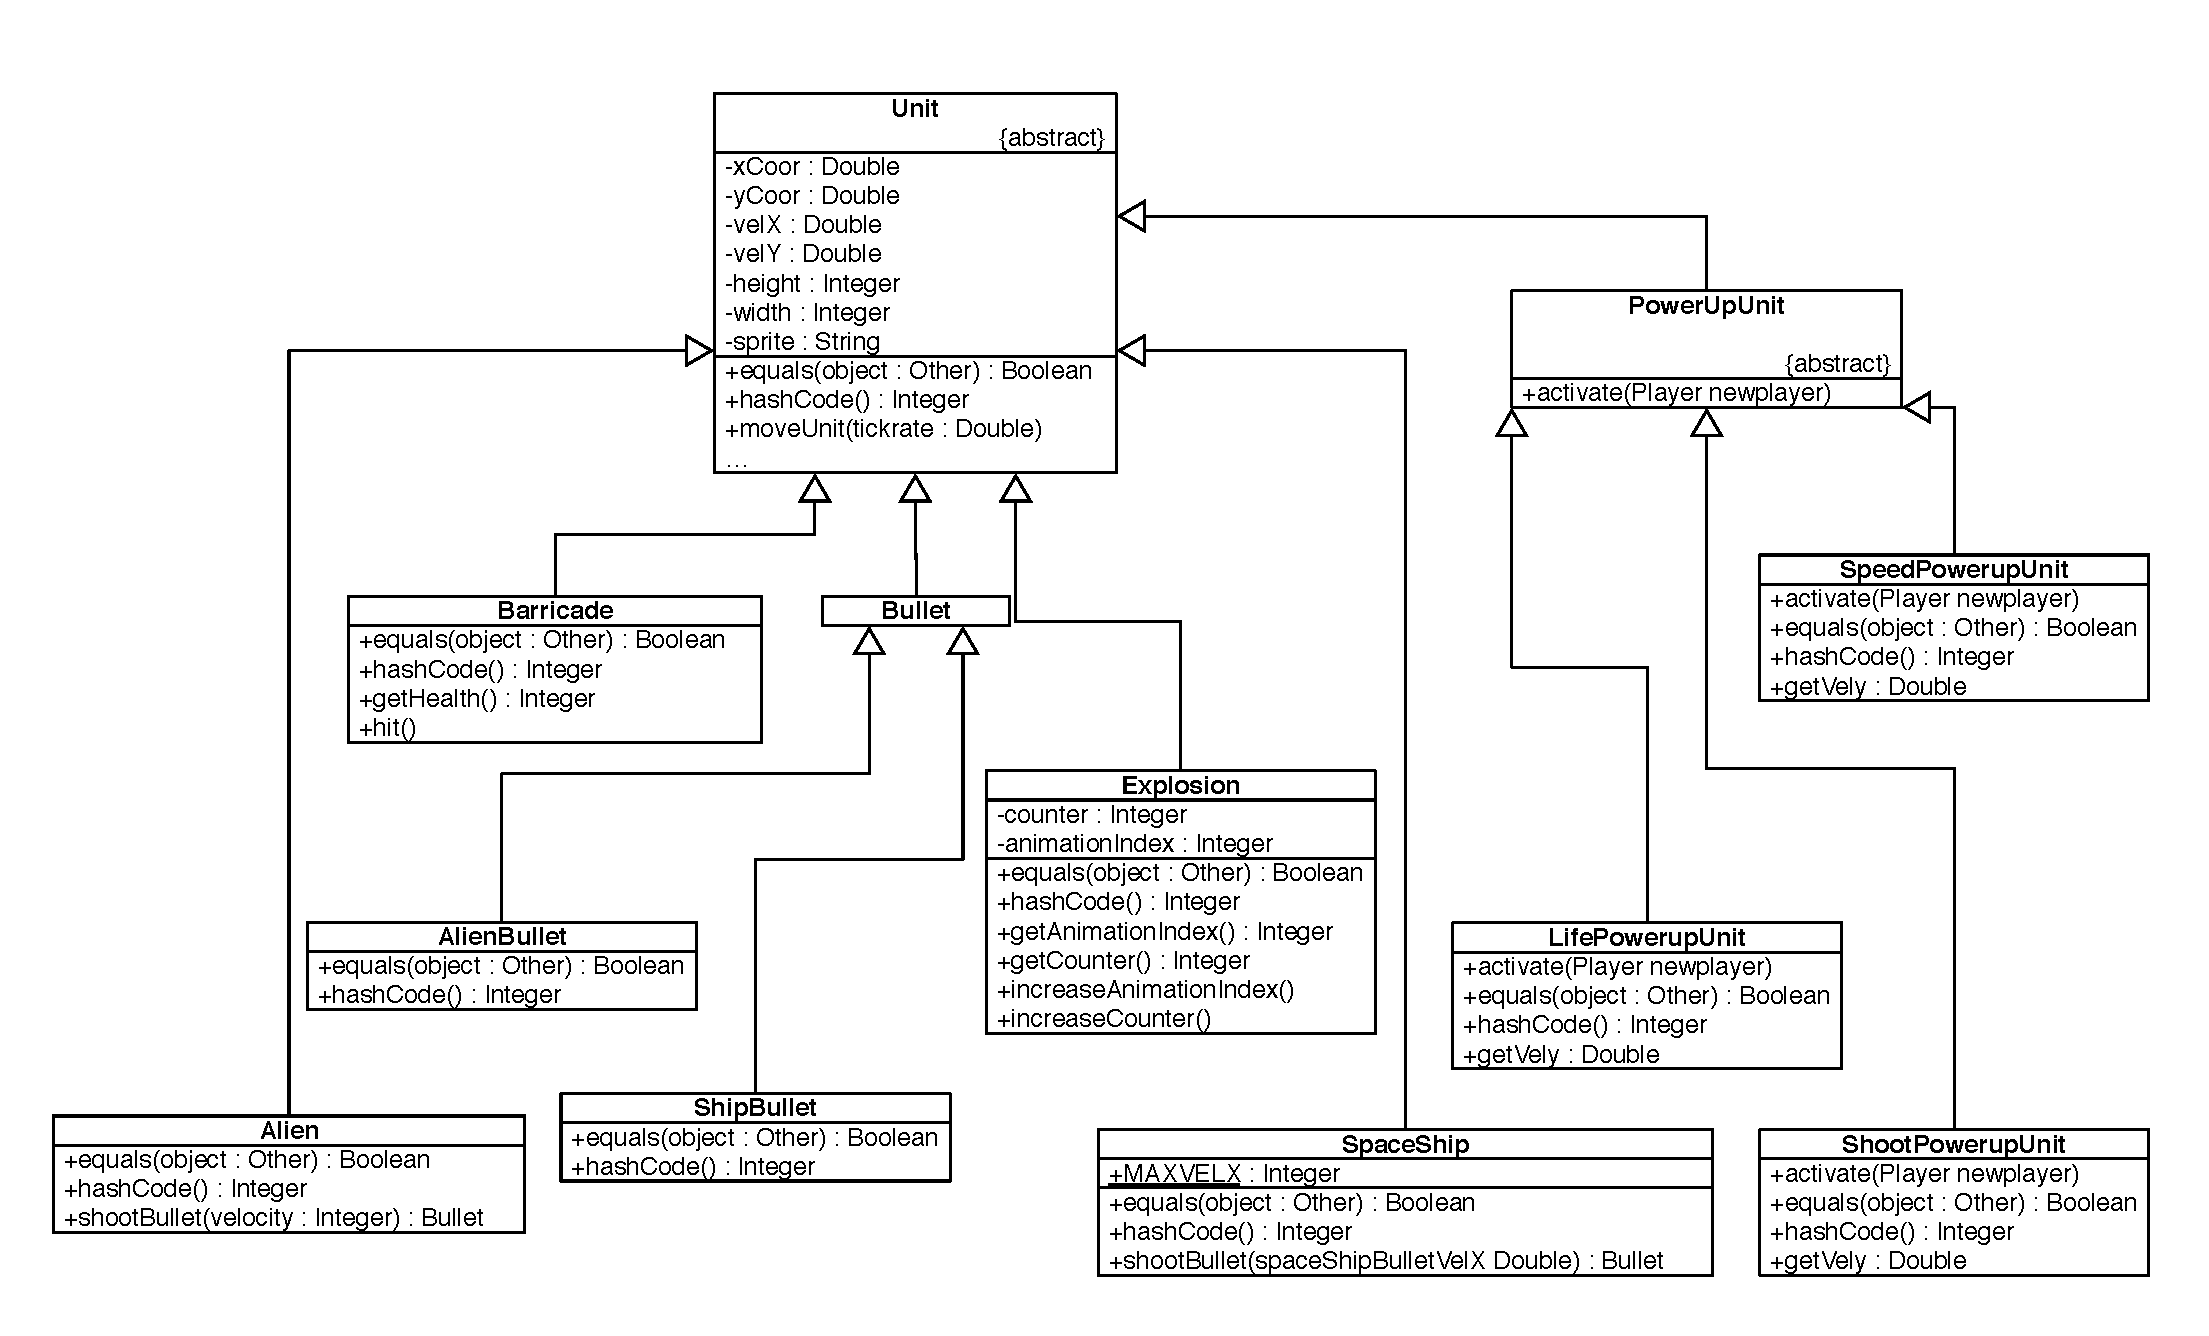
\includegraphics[width=15cm]{SI-UMLpowerupHierarchy1.pdf}
\caption{Unit UML Class Diagram}
\end{figure}
\begin{figure}[ht!]
\centering
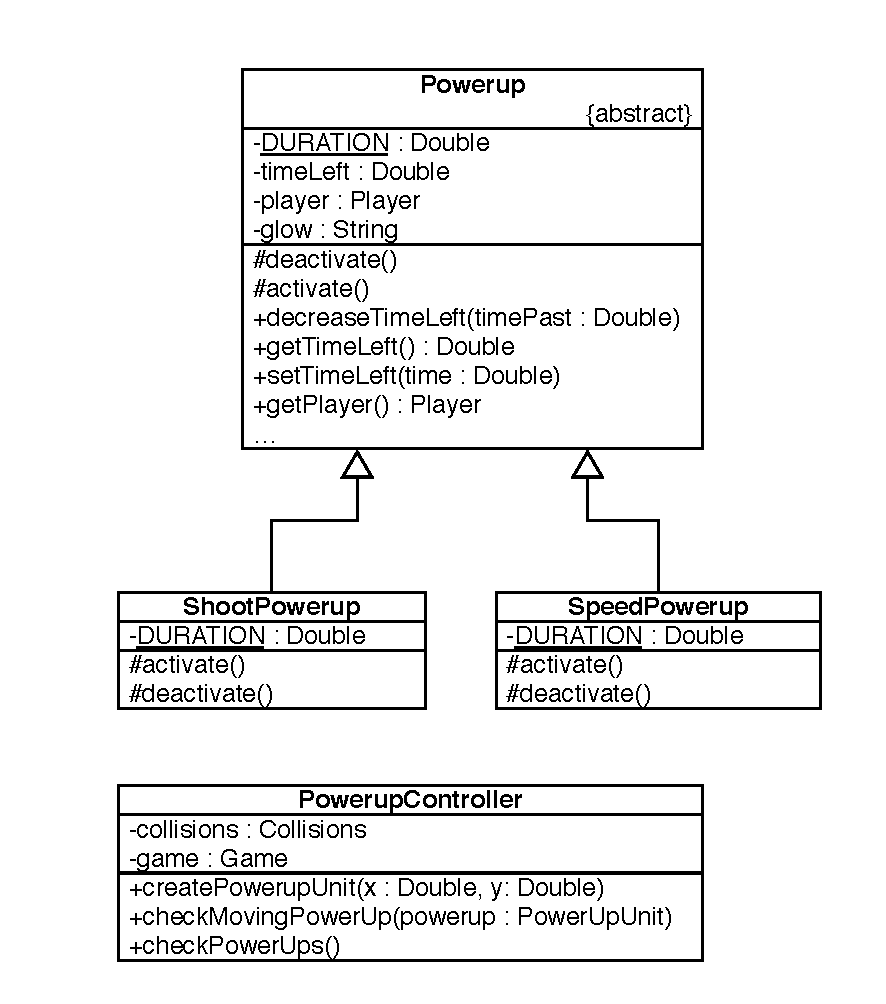
\includegraphics[width=12cm]{SI-UMLpowerupHierarchy2.pdf}
\caption{Powerup UML Class Diagram}
\end{figure}
\clearpage
\section{Powerup Functional Requirements}

A list of functional requirements considered for the implementation of powerups using the MoSCoW method described in the previous section.

\subsection{Must Haves}
Powerups must meet the following requirements:
\begin{itemize}
	\item Aliens shall randomly drop a powerup upon death.
	\item A Powerup buff shall be applied upon collision with the spaceship.
	\item A Powerup shall disappear upon collision with the spaceship.
\end{itemize}

\subsection{Should Haves}
Powerups should meet the following requirements:
\begin{itemize}
	\item Player velocity shall increase for a feasible amount of time upon collision with a Speed Powerup.
	\item Player shooting speed shall increase for a feasible amount of time upon collision with a Shooting Powerup.
	\item Player life shall increase upon collision with a Life Powerup.
	\item Player life shall not increase if the maximum amount of 5 lives has been reached.
	\item A Powerup shall have a custom sprite based on its type.
	\item A Powerup shall not disappear upon collision with a bullet.
	\item A Powerup shall not disappear upon collision with an alien.
\end{itemize}

\subsection{Could Haves}
Powerups could meet the following requirements:
\begin{itemize}
	\item A Powerup shall explode upon hitting a barricade.
\end{itemize}

\subsection{Would/Won't Haves}
Powerups won't meet the following requirements:
\begin{itemize}
	\item A Powerup shall explode upon colliding with a bullet.
\end{itemize}